
% !TeX spellcheck = en_GB
\documentclass{beamer}
\usepackage[utf8]{inputenc}
 \usetheme{antibes}
 \usepackage{movie15}
 \usepackage{graphicx}
 \usepackage{hyperref}
 \usepackage{tikz}
 \usetikzlibrary{shapes.geometric, arrows}
 \tikzstyle{startstop} = [rectangle, rounded corners, minimum width=3cm, minimum height=1cm,text centered, draw=blue, fill=blue!15]
 \tikzstyle{arrow} = [thick,->,>=stealth]
 \hypersetup{
 	colorlinks=true,
 	linkcolor=blue,
 	filecolor=magenta,      
 	urlcolor=cyan,
 }
 
 \urlstyle{same}
 \title[\textcolor{orange}{}] %optional
 {Application of Hilbert-Huang Transform to Bearing Fault Detection}
 
 \subtitle{} 
 \author[] % (optional, for multiple authors)
 {Yapi Donatien Achou}
 
% \institute[VFU] % (optional)
% {
% 	\inst{1}%
% 	Faculty of Physics\\
% 	Very Famous University
% 	\and
% 	\inst{2}%
% 	Faculty of Chemistry\\
% 	Very Famous University
% }
 
 %\date[VLC 2013] % (optional)
 %{Very Large Conference, April 2013}
 
 \logo{
\includegraphics[height=1.5cm]{uib}}
 
 
\begin{document}
 
\frame{\titlepage}
 
 
 %%%%%%%%%%%%%%%%%%%%%%%%%%%%%%%%%%%%%%%%%%%%%%%%%%%%%%%%%%%
 
 
 
 %%%%%%%%%%%%%%%%%%%%%%%%%%%%%%%%%%%%%%%%%%%%%%%%%%%%%%%%%%%%
 
\begin{frame}
\frametitle{Bearings facilitate rotation movements}
\begin{figure}[H]
	\centering
	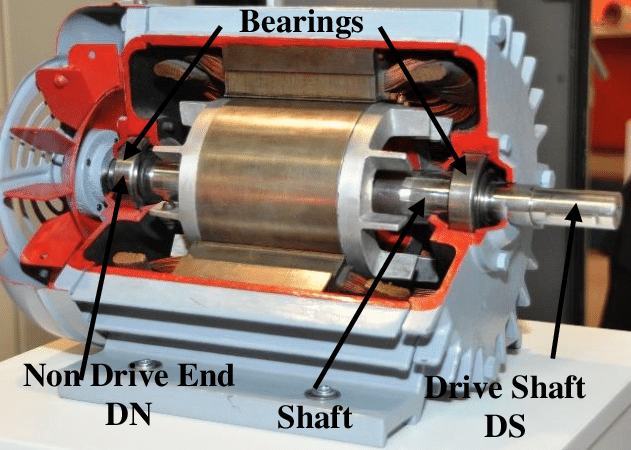
\includegraphics[width=0.8\linewidth]{motor}
	%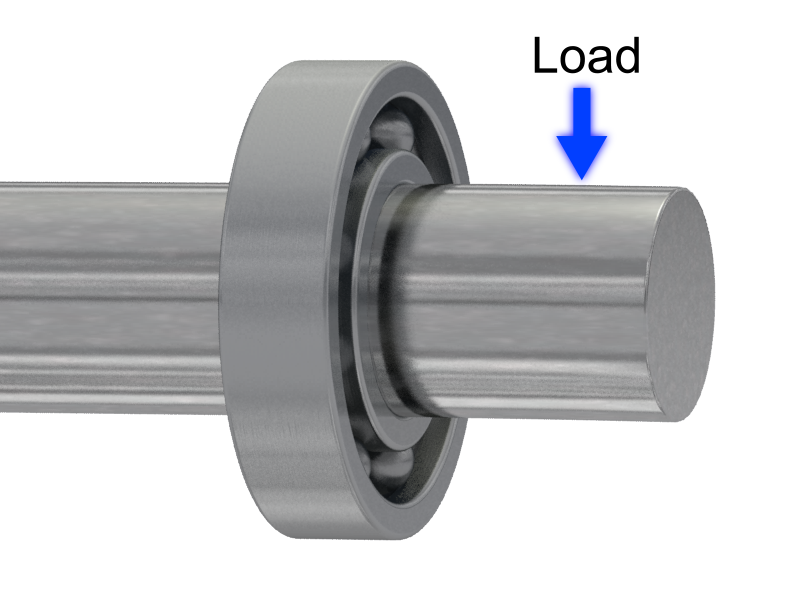
\includegraphics[width=0.4\linewidth]{bearing}
	%\caption{}
	%\label{fig:datascience}
\end{figure}
\end{frame}
%%%%%%%%%%%%%%%%%%%%%%%%%%%%%%%%%%%%%%%%%%%%%%%%%%%%%%
\begin{frame}
	\frametitle{A bearing has multiple components}
	\begin{figure}[H]
		\centering
		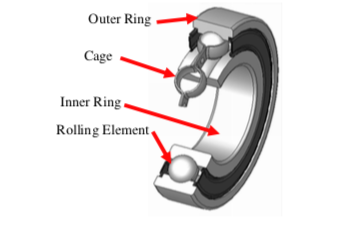
\includegraphics[width=0.5\linewidth]{bearing-geometry1}
		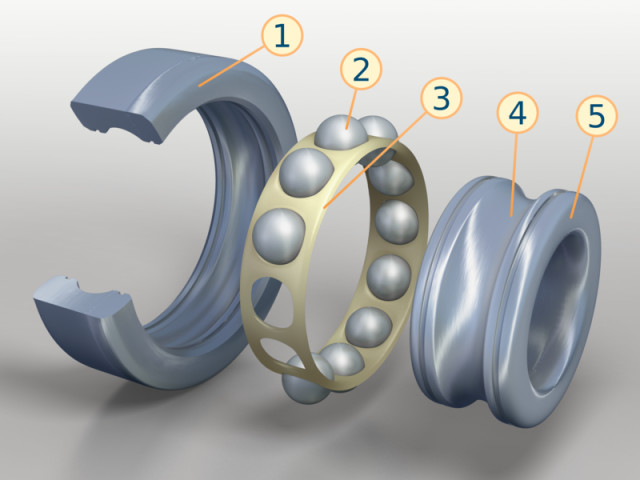
\includegraphics[width=0.5\linewidth]{bearing-geometry2}
		%\caption{}
		%\label{fig:datascience}
	\end{figure}
\end{frame}

%%%%%%%%%%%%%%%%%%%%%%%%%%%%%%%%%%%%%%%%%%%%%%%%%%%%%%

%\begin{frame}
%	\frametitle{Introduction to bearings}
%	\begin{figure}[H]
%		\centering
%		%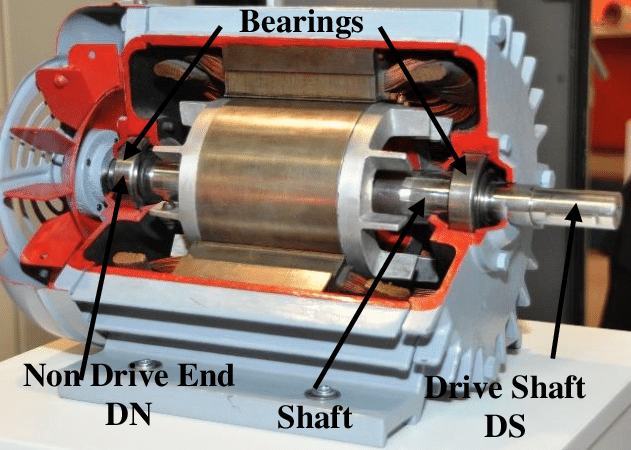
\includegraphics[width=0.8\linewidth]{motor}
%		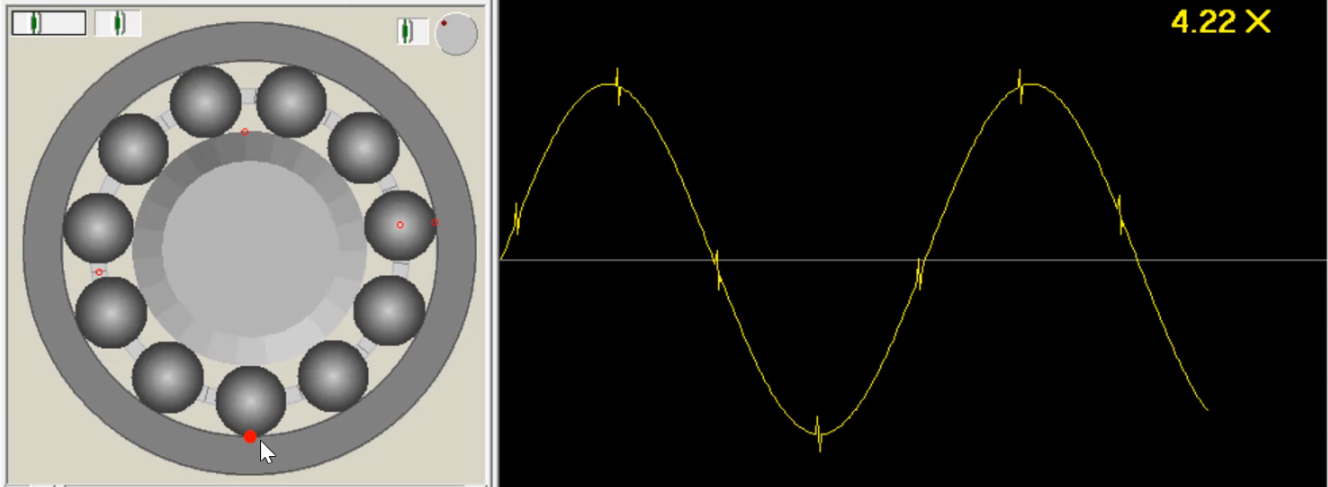
\includegraphics[width=0.8\linewidth]{outer-race1}
%		%\caption{}
%		%\label{fig:datascience}
%	\end{figure}
%\end{frame}

%%%%%%%%%%%%%%%%%%%%%%%%%%%%%%%%%%%%%%%%%%%%%%%%%%%%%%

\begin{frame}
	\frametitle{Bearings are subjected to large forces}
	\begin{figure}[H]
		\centering
		%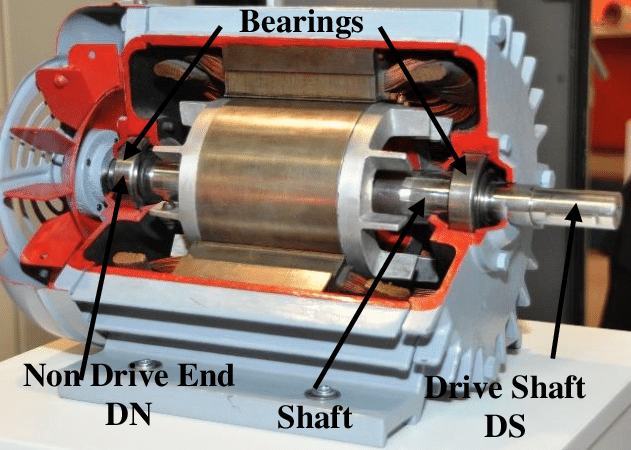
\includegraphics[width=0.8\linewidth]{motor}
		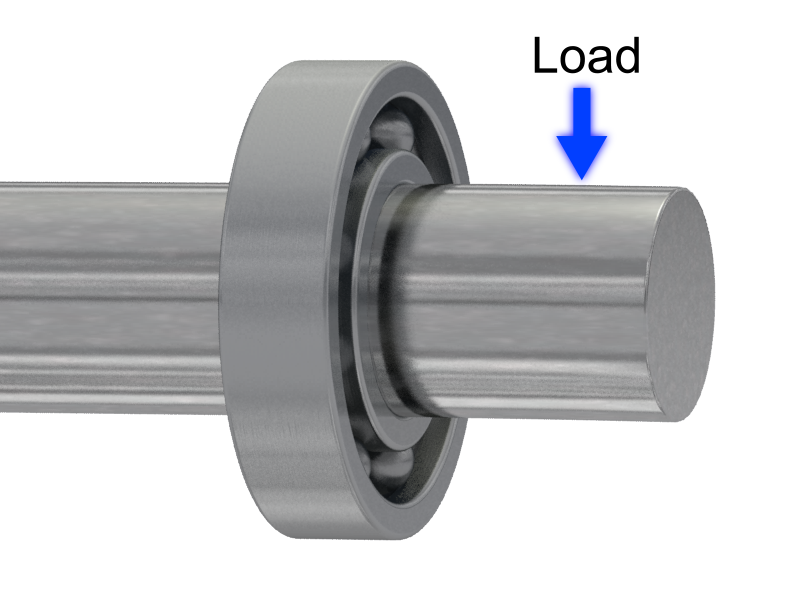
\includegraphics[width=0.8\linewidth]{bearing}
		%\caption{}
		%\label{fig:datascience}
	\end{figure}
\end{frame}

%%%%%%%%%%%%%%%%%%%%%%%%%%%%%%%%%%%%%%%%%%%%%%%%%%%%%%%%

\begin{frame}
	\frametitle{Fault can result as a consequences of load}
	\begin{figure}[H]
		\centering
		%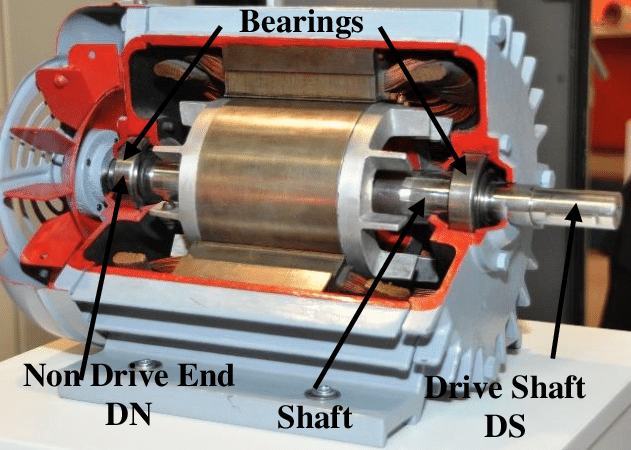
\includegraphics[width=0.8\linewidth]{motor}
		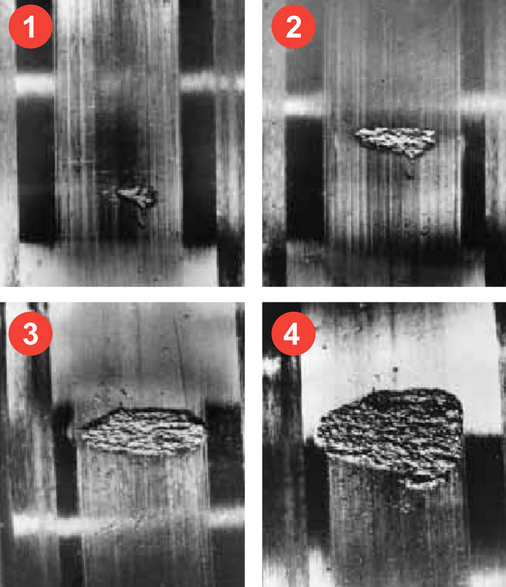
\includegraphics[width=0.6\linewidth]{bearing_fault_evolution}
		%\caption{}
		%\label{fig:datascience}
	\end{figure}
\end{frame}
%%%%%%%%%%%%%%%%%%%%%%%%%%%%%%%%%%%%%%%%%%%%%%%%%%%%%%%%

%%%%%%%%%%%%%%%%%%%%%%%%%%%%%%%%%%%%%%%%%%%%%%%%%%%%%%%%

\begin{frame}
	\frametitle{Bearing faults depends on their physical characteristics}
\begin{equation}
	BPFI = \frac{nb}{2}R\left(  1+ \frac{BD}{PD}\cos(\beta) \right)
\end{equation}

\begin{equation}
BPFO = \frac{nb}{2}R\left(  1- \frac{BD}{PD}\cos(\beta) \right)
\end{equation}
\end{frame}
%%%%%%%%%%%%%%%%%%%%%%%%%%%%%%%%%%%%%%%%%%%%%%%%%%%%%%%%




\begin{frame}
	\frametitle{Bearing faults generate high frequency shock and amplitude modulates the raw vibration signal}
	\begin{figure}[H]
		\centering
		%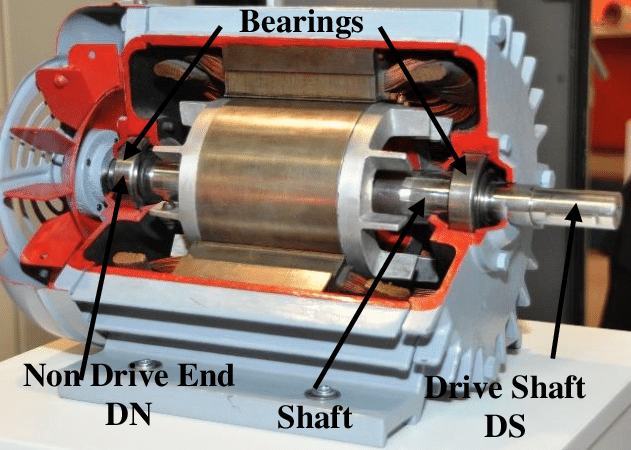
\includegraphics[width=0.8\linewidth]{motor}
		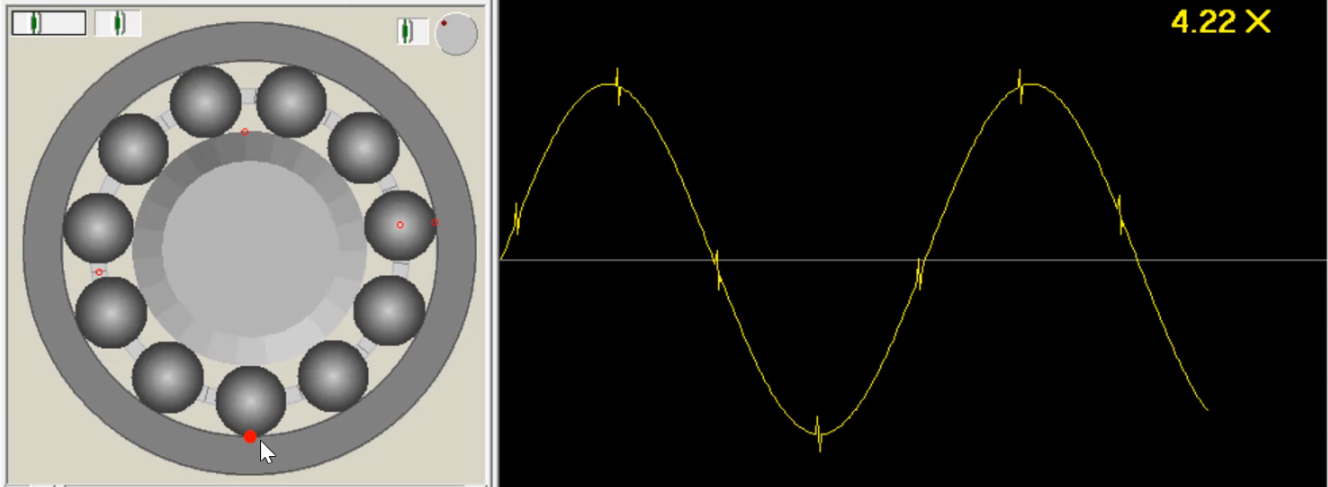
\includegraphics[width=0.5\linewidth]{outer-race1}
		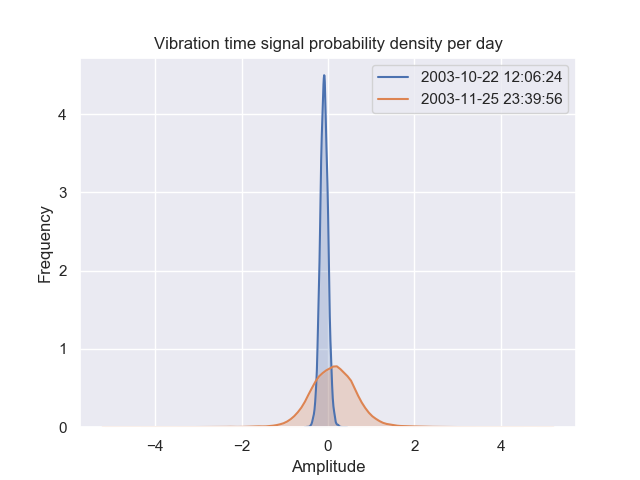
\includegraphics[width=0.6\linewidth]{bpfi_density}
		%\caption{}
		%\label{fig:datascience}
	\end{figure}
\end{frame}

%%%%%%%%%%%%%%%%%%%%%%%%%%%%%%%%%%%%%%%%%%%%%%%%%%%%%%%%
\begin{frame}
	\frametitle{Bearings inner race and outer race shock are different}
	\begin{figure}[H]
		\centering
		%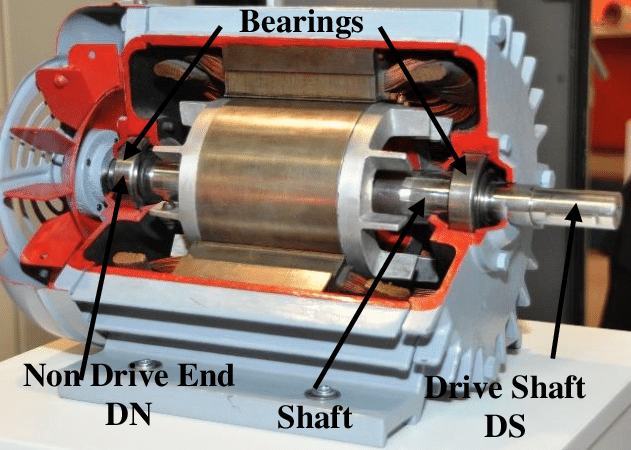
\includegraphics[width=0.8\linewidth]{motor}
		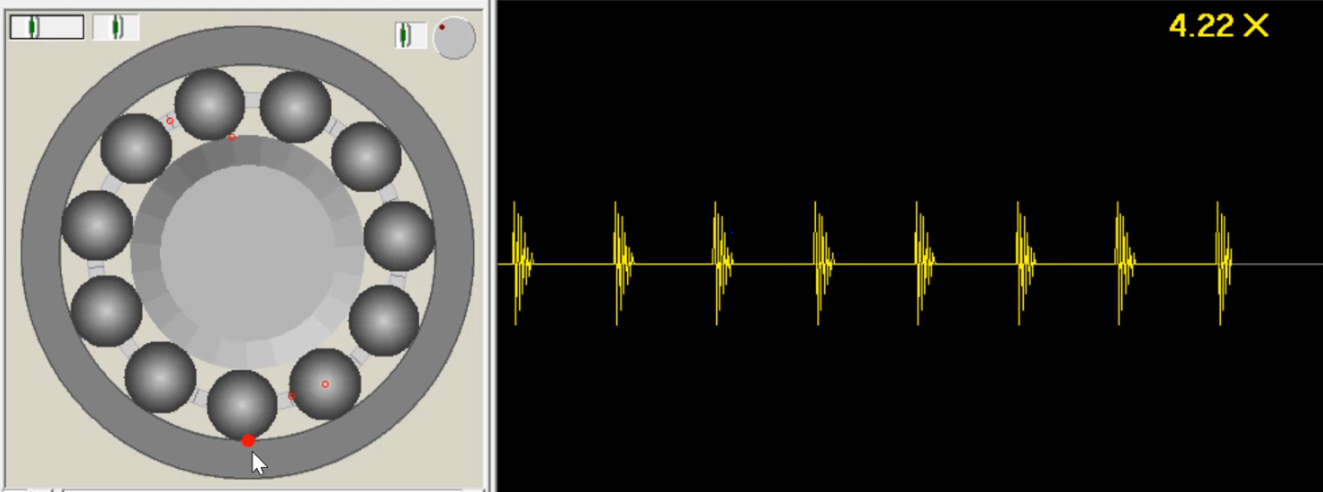
\includegraphics[width=0.8\linewidth]{outer-race2}
		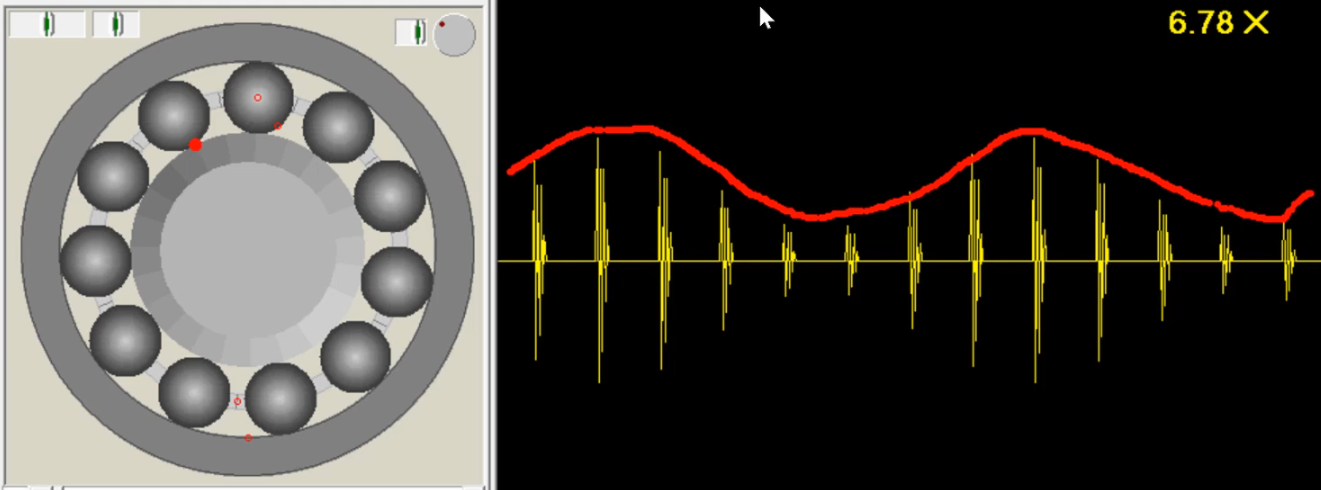
\includegraphics[width=0.8\linewidth]{inner-race2}
		%\caption{}
		%\label{fig:datascience}
	\end{figure}
\end{frame}

%%%%%%%%%%%%%%%%%%%%%%%%%%%%%%%%%%%%%%%%%%%%%%%%%%%%%%%%%



%%%%%%%%%%%%%%%%%%%%%%%%%%%%%%%%%%%%%%%%%%%%%%%%%%%%%%%%
\begin{frame}
	\frametitle{The High frequency Resonance Technique isolates bearing faults }
	\begin{figure}[H]
		\centering
		%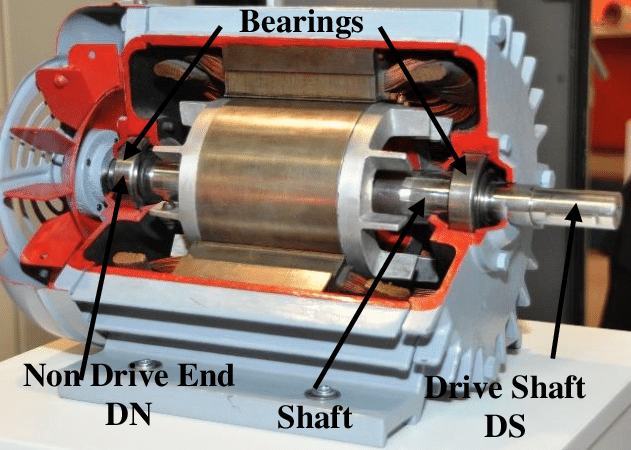
\includegraphics[width=0.8\linewidth]{motor}
		%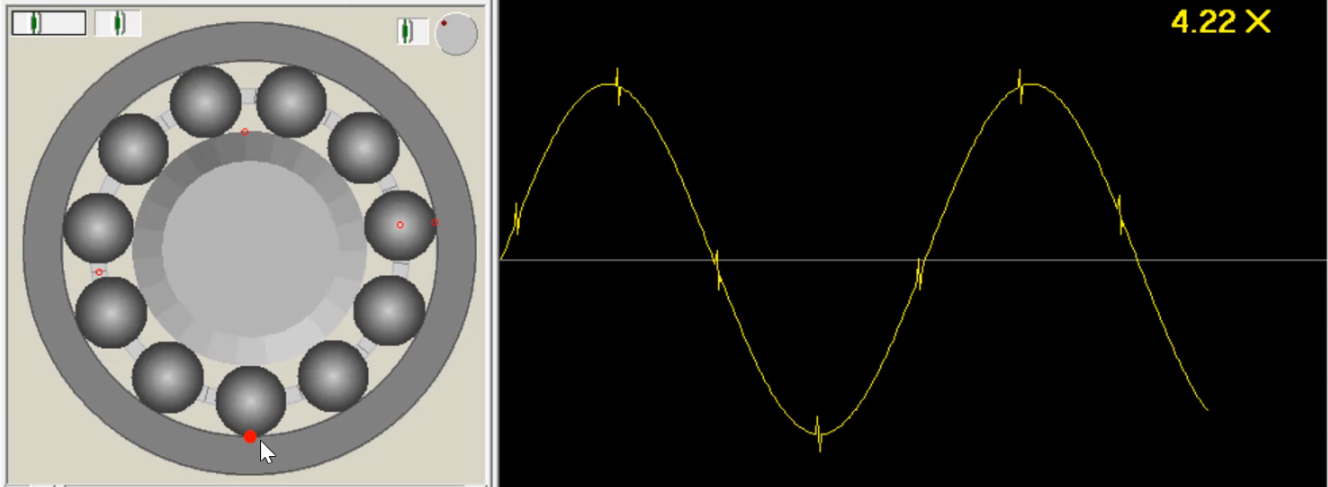
\includegraphics[width=0.8\linewidth]{outer-race1}
		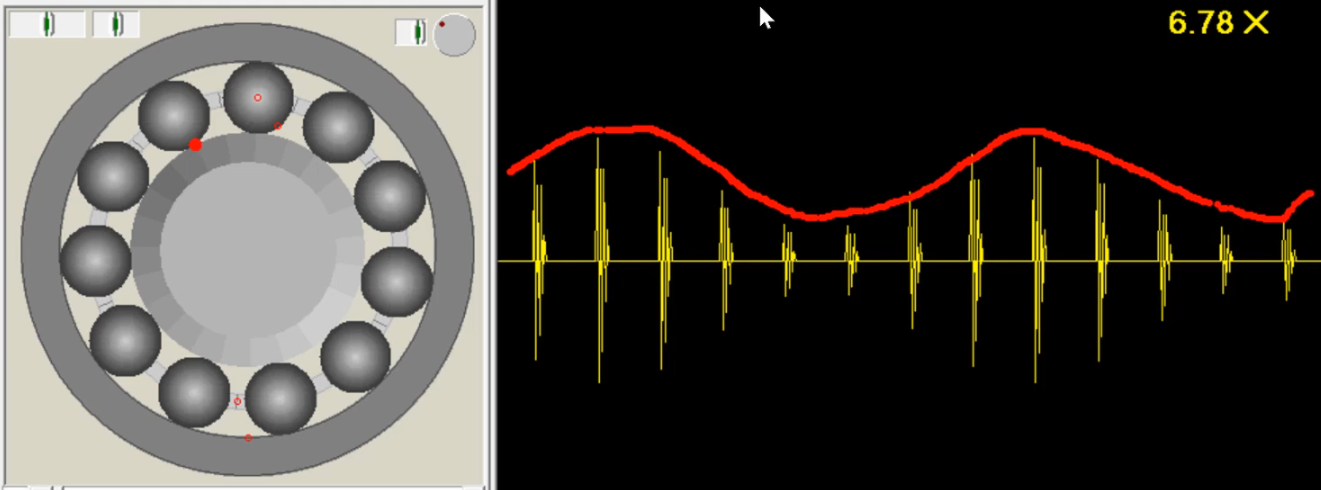
\includegraphics[width=1.\linewidth]{inner-race2}
		%\caption{}
		%\label{fig:datascience}
	\end{figure}
\end{frame}

%%%%%%%%%%%%%%%%%%%%%%%%%%%%%%%%%%%%%%%%%%%%%%%%%%%%%%%%%

%%%%%%%%%%%%%%%%%%%%%%%%%%%%%%%%%%%%%%%%%%%%%%%%%%%%%%%%
\begin{frame}
	\frametitle{The High frequency Resonance Technique filters a target vibration signal}
	\begin{figure}[H]
		\centering
		
		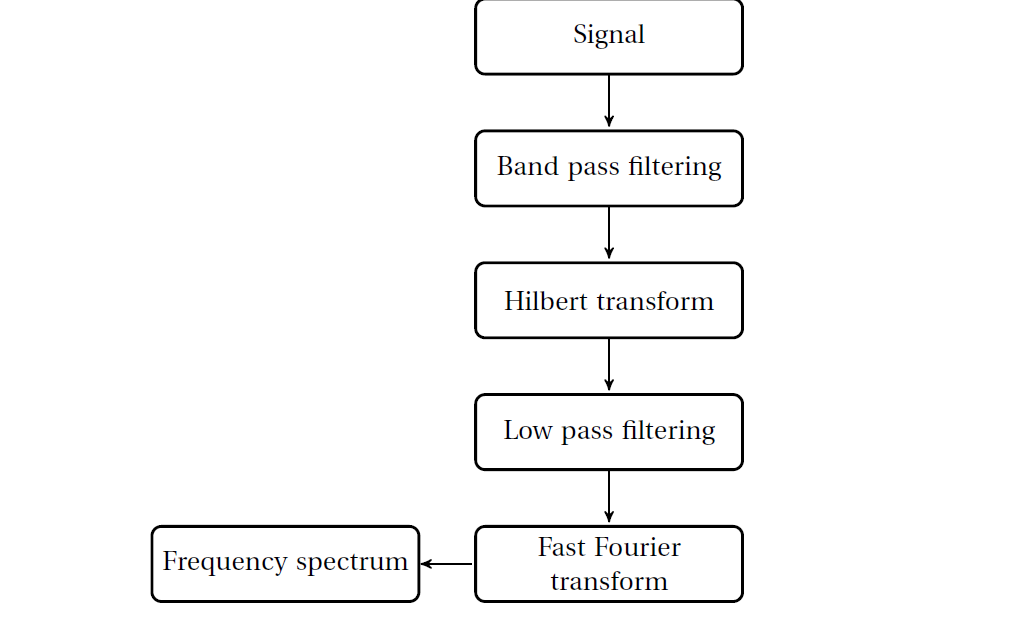
\includegraphics[width=0.8\linewidth]{hfrt}
		%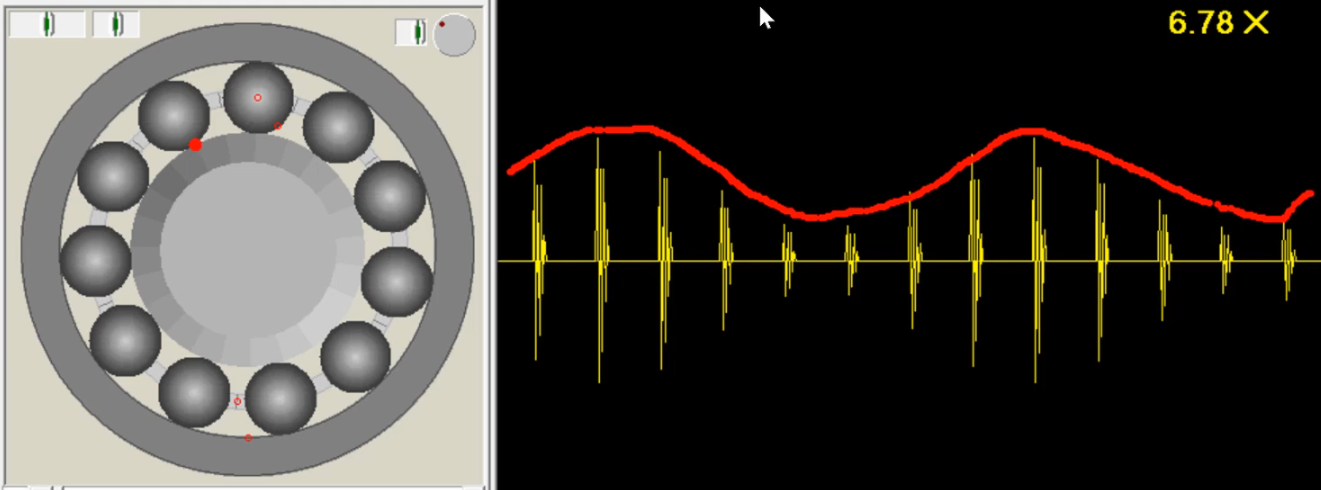
\includegraphics[width=0.8\linewidth]{inner-race2}
		%\caption{}
		%\label{fig:datascience}
	\end{figure}
\end{frame}

%%%%%%%%%%%%%%%%%%%%%%%%%%%%%%%%%%%%%%%%%%%%%%%%%%%%%%%%%

%%%%%%%%%%%%%%%%%%%%%%%%%%%%%%%%%%%%%%%%%%%%%%%%%%%%%%%%
\begin{frame}
	\frametitle{The Hilbert transform extracts the envelop of the filtered signal }
	\begin{equation}
		H(s(t)) = \frac{1}{\pi t}*s(t) = \frac{1}{\pi}P\int_{-\infty}^{+\infty}\frac{s(\eta)}{t-\eta}d\eta
	\end{equation}
	
	\begin{equation}
		y(t) = s(t) + iH(s(t))
	\end{equation}
	
	\begin{equation}
Envelop(s(t)) = \sqrt{s(t)^{2} + H(s(t))^{2}} 
	\end{equation}
	
	\begin{figure}[H]
		\centering
		
		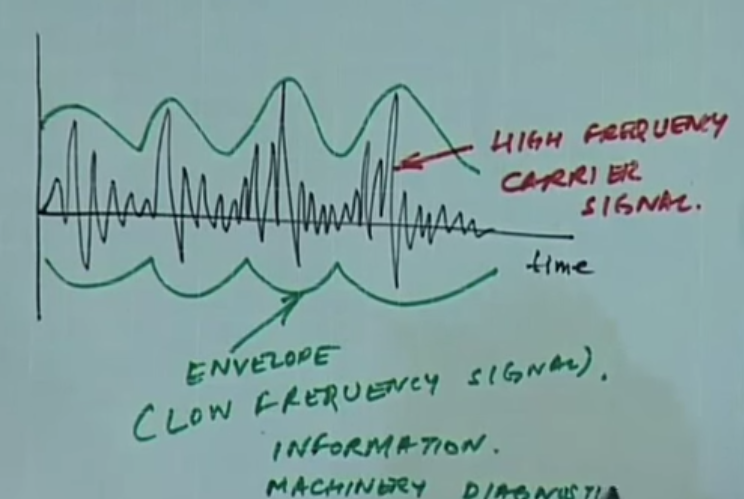
\includegraphics[width=0.4\linewidth]{env}
		%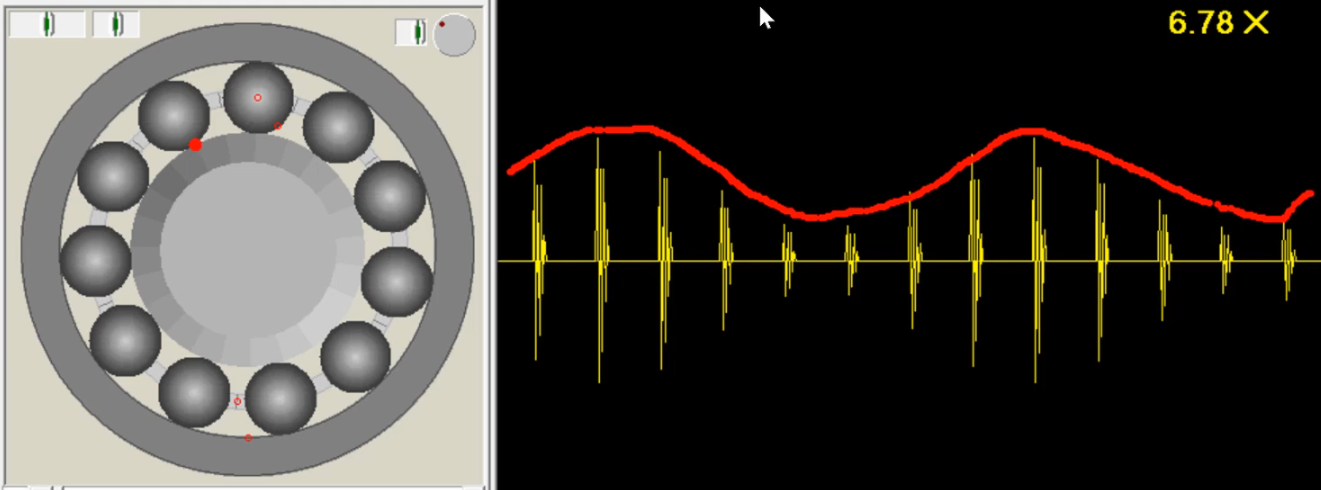
\includegraphics[width=0.8\linewidth]{inner-race2}
		%\caption{}
		%\label{fig:datascience}
	\end{figure}
	
\end{frame}

%%%%%%%%%%%%%%%%%%%%%%%%%%%%%%%%%%%%%%%%%%%%%%%%%%%%%%%%%


%%%%%%%%%%%%%%%%%%%%%%%%%%%%%%%%%%%%%%%%%%%%%%%%%%%%%%%%
\begin{frame}
	\frametitle{A bearing fault is revealed through the Fourier transform}
	\begin{figure}[H]
		\centering
		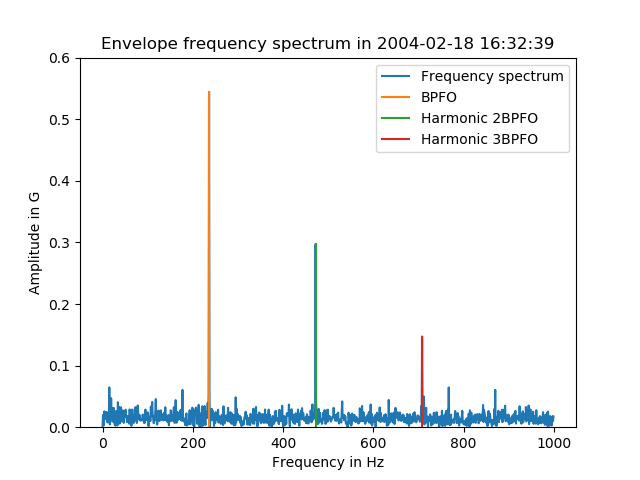
\includegraphics[width=0.45\linewidth]{last_day_spectrum_bpfo}
		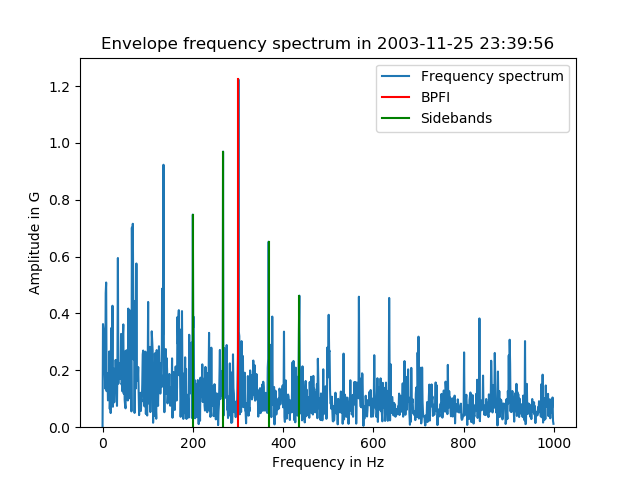
\includegraphics[width=0.45\linewidth]{bpfi_sidebands}
		%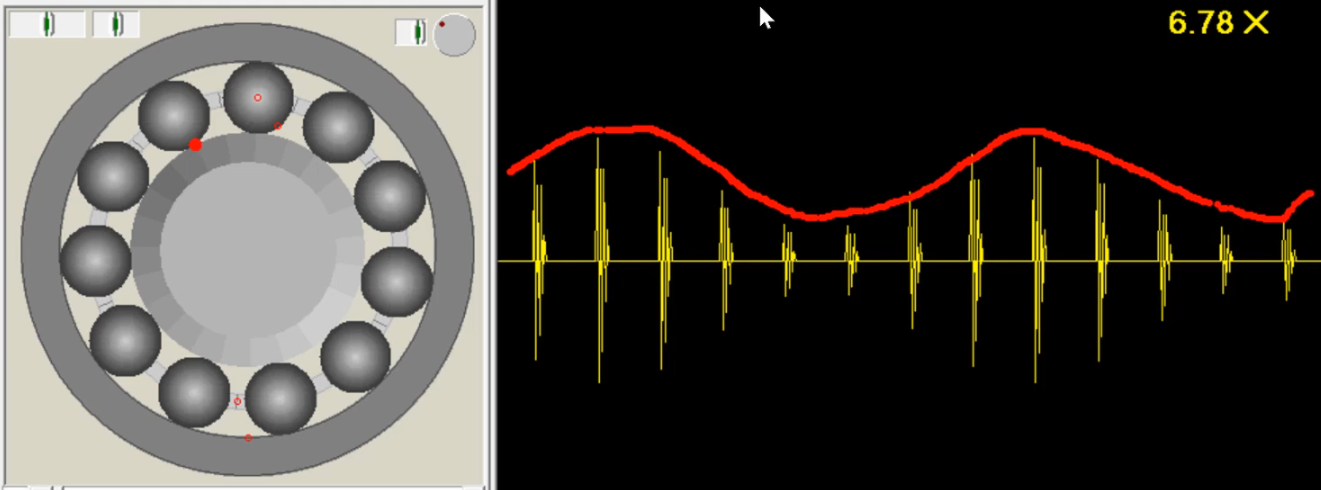
\includegraphics[width=0.8\linewidth]{inner-race2}
		%\caption{}
		%\label{fig:datascience}
	\end{figure}
\end{frame}

%%%%%%%%%%%%%%%%%%%%%%%%%%%%%%%%%%%%%%%%%%%%%%%%%%%%%%%%%


%%%%%%%%%%%%%%%%%%%%%%%%%%%%%%%%%%%%%%%%%%%%%%%%%%%%%%%%
\begin{frame}
	\frametitle{A bearing fault grows exponentially}
	\begin{figure}[H]
		\centering
		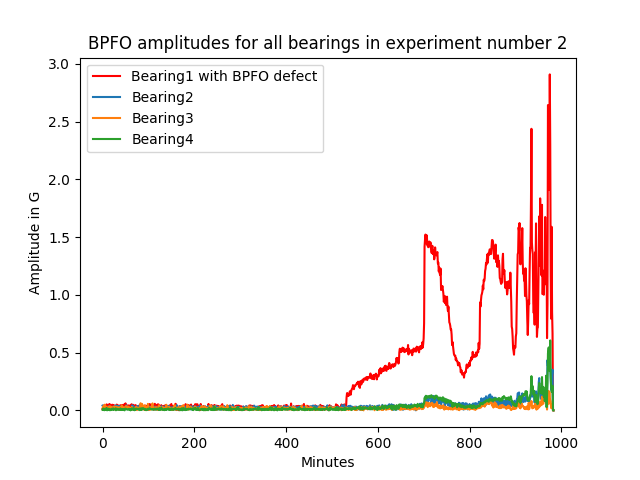
\includegraphics[width=0.45\linewidth]{bpfo}
		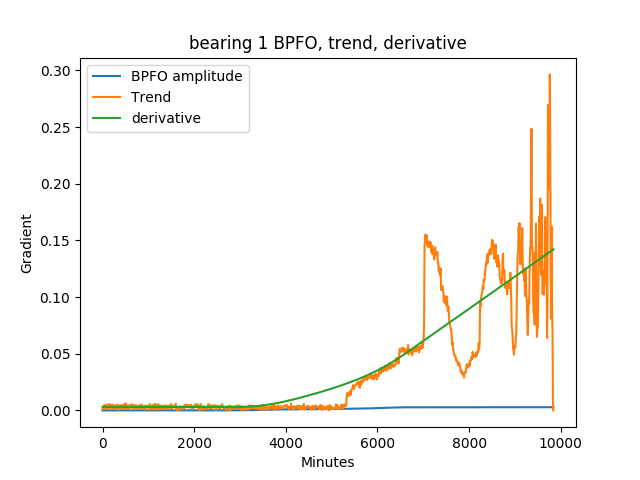
\includegraphics[width=0.45\linewidth]{exp}
		%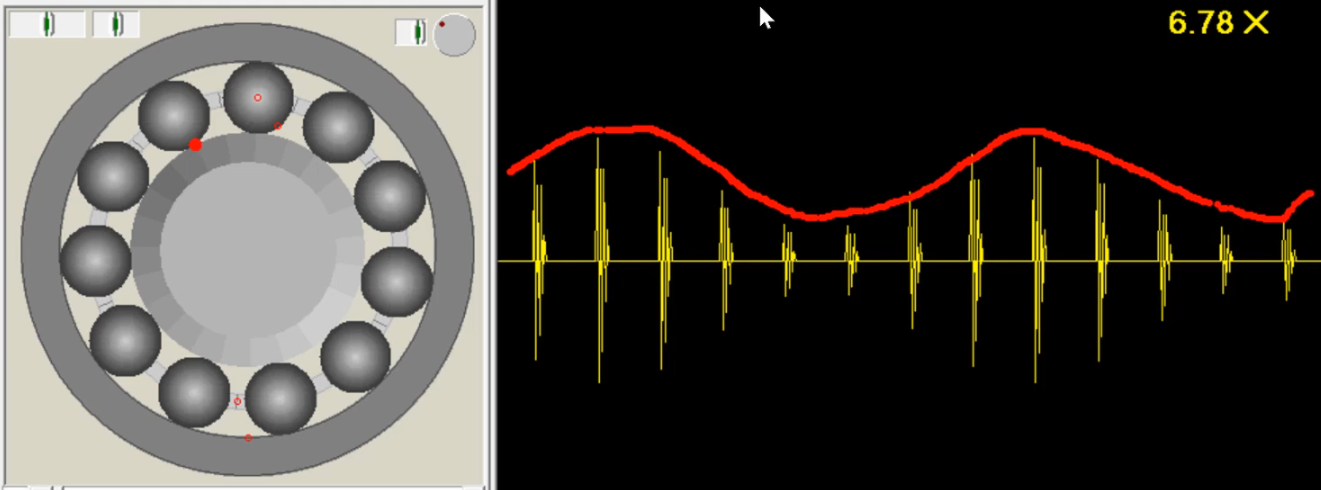
\includegraphics[width=0.8\linewidth]{inner-race2}
		%\caption{}
		%\label{fig:datascience}
	\end{figure}
\end{frame}

%%%%%%%%%%%%%%%%%%%%%%%%%%%%%%%%%%%%%%%%%%%%%%%%%%%%%%%%%

%%%%%%%%%%%%%%%%%%%%%%%%%%%%%%%%%%%%%%%%%%%%%%%%%%%%%%%%
\begin{frame}
	\frametitle{The High Frequency Resonance Technique can produce a noisy spectrum for fault in the inner race}
	\begin{figure}[H]
		\centering
		%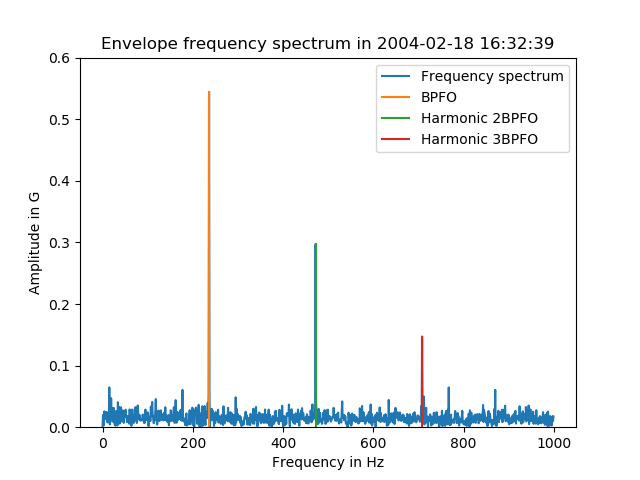
\includegraphics[width=0.45\linewidth]{last_day_spectrum_bpfo}
		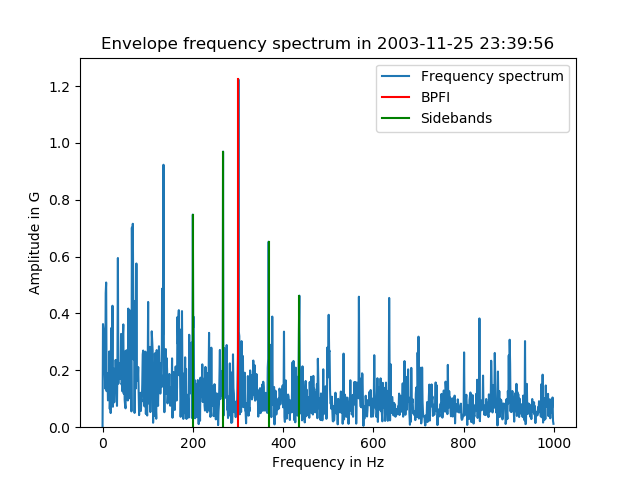
\includegraphics[width=0.8\linewidth]{bpfi_sidebands}
		%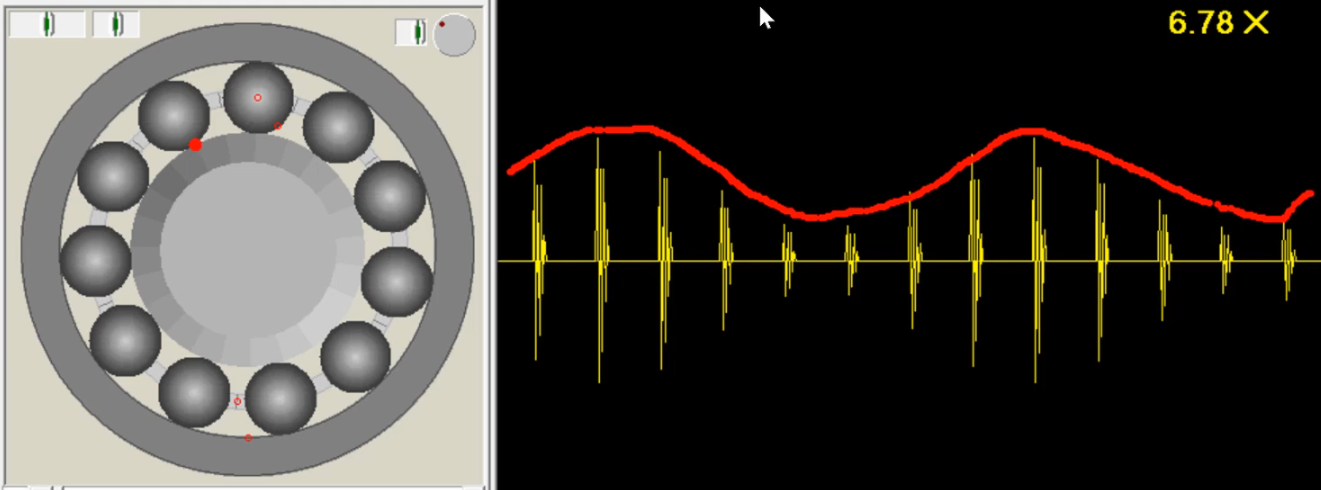
\includegraphics[width=0.8\linewidth]{inner-race2}
		%\caption{}
		%\label{fig:datascience}
	\end{figure}
\end{frame}

%%%%%%%%%%%%%%%%%%%%%%%%%%%%%%%%%%%%%%%%%%%%%%%%%%%%%%%%%
%%%%%%%%%%%%%%%%%%%%%%%%%%%%%%%%%%%%%%%%%%%%%%%%%%%%%%%%
\begin{frame}
	\frametitle{Advantage and disadvantage of the Fourier Transform}
	\begin{itemize}
		\item \textcolor{green}{Recovers frequency content of a signal}
		\item \textcolor{orange}{Valid in the frequency domain}
		\item \textcolor{orange}{Ignores events}
	\end{itemize}
\end{frame}

%%%%%%%%%%%%%%%%%%%%%%%%%%%%%%%%%%%%%%%%%%%%%%%%%%%%%%%%%


%%%%%%%%%%%%%%%%%%%%%%%%%%%%%%%%%%%%%%%%%%%%%%%%%%%%%%%%
\begin{frame}
	\frametitle{Hilbert-Huang Transform for bearing fault detection}
	\begin{figure}[H]
		\centering
		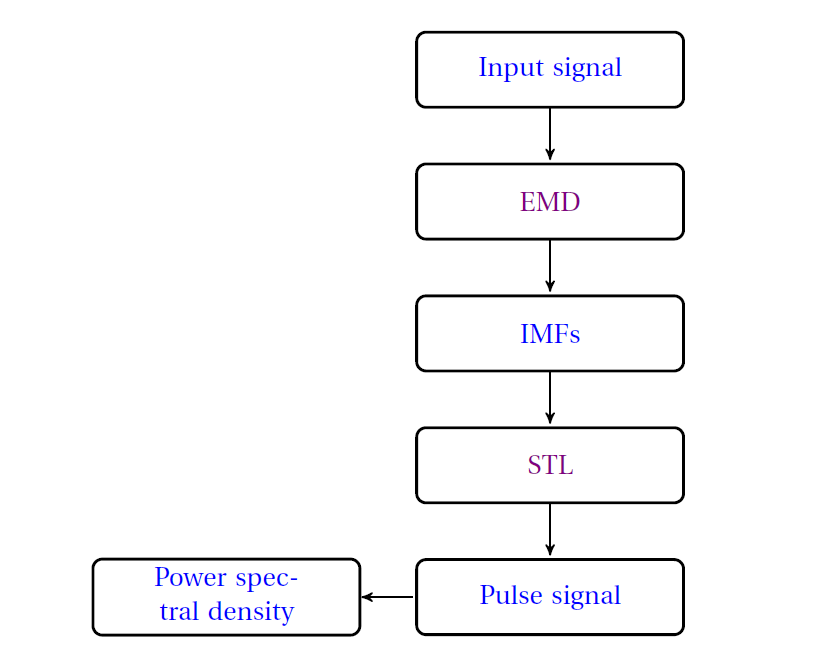
\includegraphics[width=0.8\linewidth]{new_method}
		%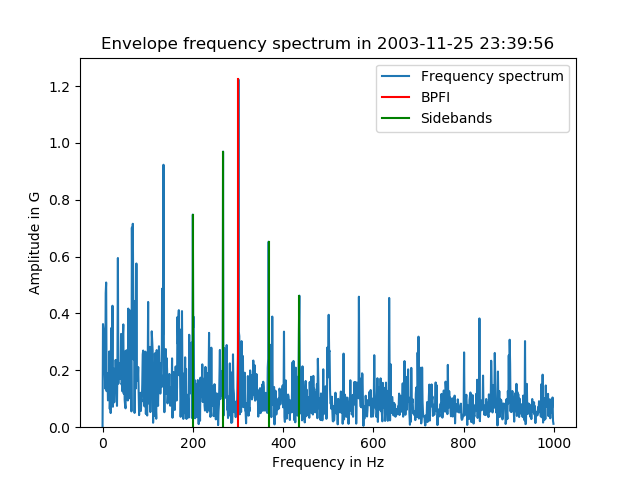
\includegraphics[width=0.45\linewidth]{bpfi_sidebands}
		%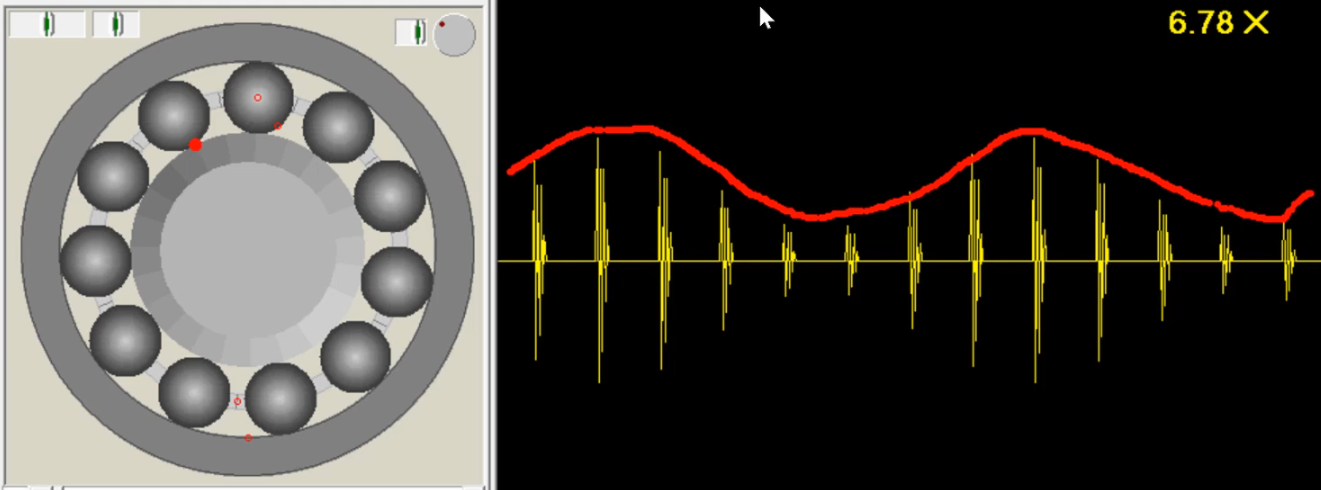
\includegraphics[width=0.8\linewidth]{inner-race2}
		%\caption{}
		%\label{fig:datascience}
	\end{figure}
\end{frame}

%%%%%%%%%%%%%%%%%%%%%%%%%%%%%%%%%%%%%%%%%%%%%%%%%%%%%%%%%
%%%%%%%%%%%%%%%%%%%%%%%%%%%%%%%%%%%%%%%%%%%%%%%%%%%%%%%%
\begin{frame}
	\frametitle{The Hilbert-Huang transform (HHT) splits a signal into Intrinsic Mode Function(IMF)}
		\begin{equation}
	c_{j} = \sum_{j=1}^{N}s_{j}(t) + r(t)
	\end{equation}
	\begin{figure}[H]
		\centering
		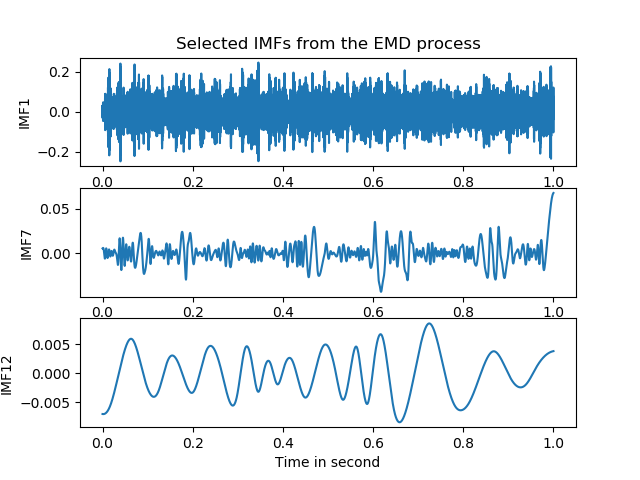
\includegraphics[width=0.6\linewidth]{selected_imf}
		%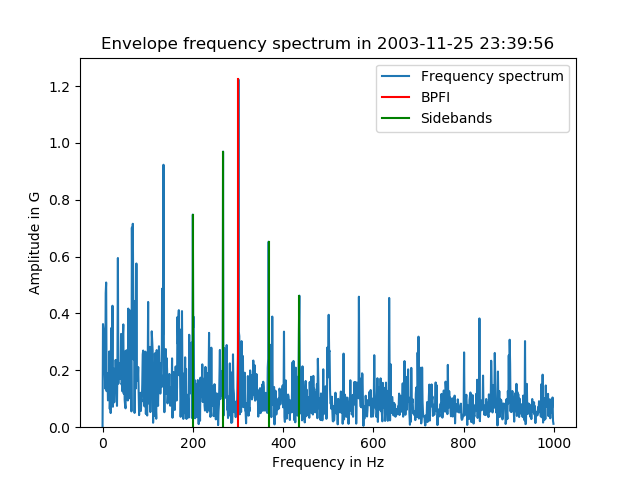
\includegraphics[width=0.45\linewidth]{bpfi_sidebands}
		%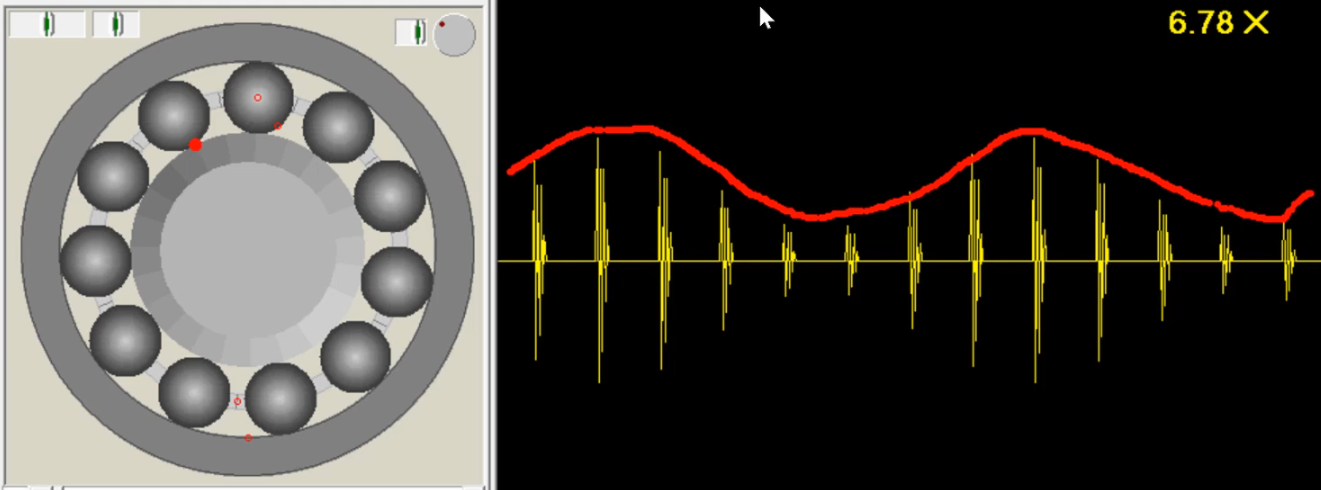
\includegraphics[width=0.8\linewidth]{inner-race2}
		%\caption{}
		%\label{fig:datascience}
	\end{figure}
\end{frame}

%%%%%%%%%%%%%%%%%%%%%%%%%%%%%%%%%%%%%%%%%%%%%%%%%%%%%%%%%
%%%%%%%%%%%%%%%%%%%%%%%%%%%%%%%%%%%%%%%%%%%%%%%%%%%%%%%%
\begin{frame}
	\frametitle{The Seasonal Trend Decomposition (STL) extracts cyclical components }
	\begin{equation}
		s(t) = T(t) + C(t) + T(t)
	\end{equation}
	\begin{figure}[H]
		\centering
		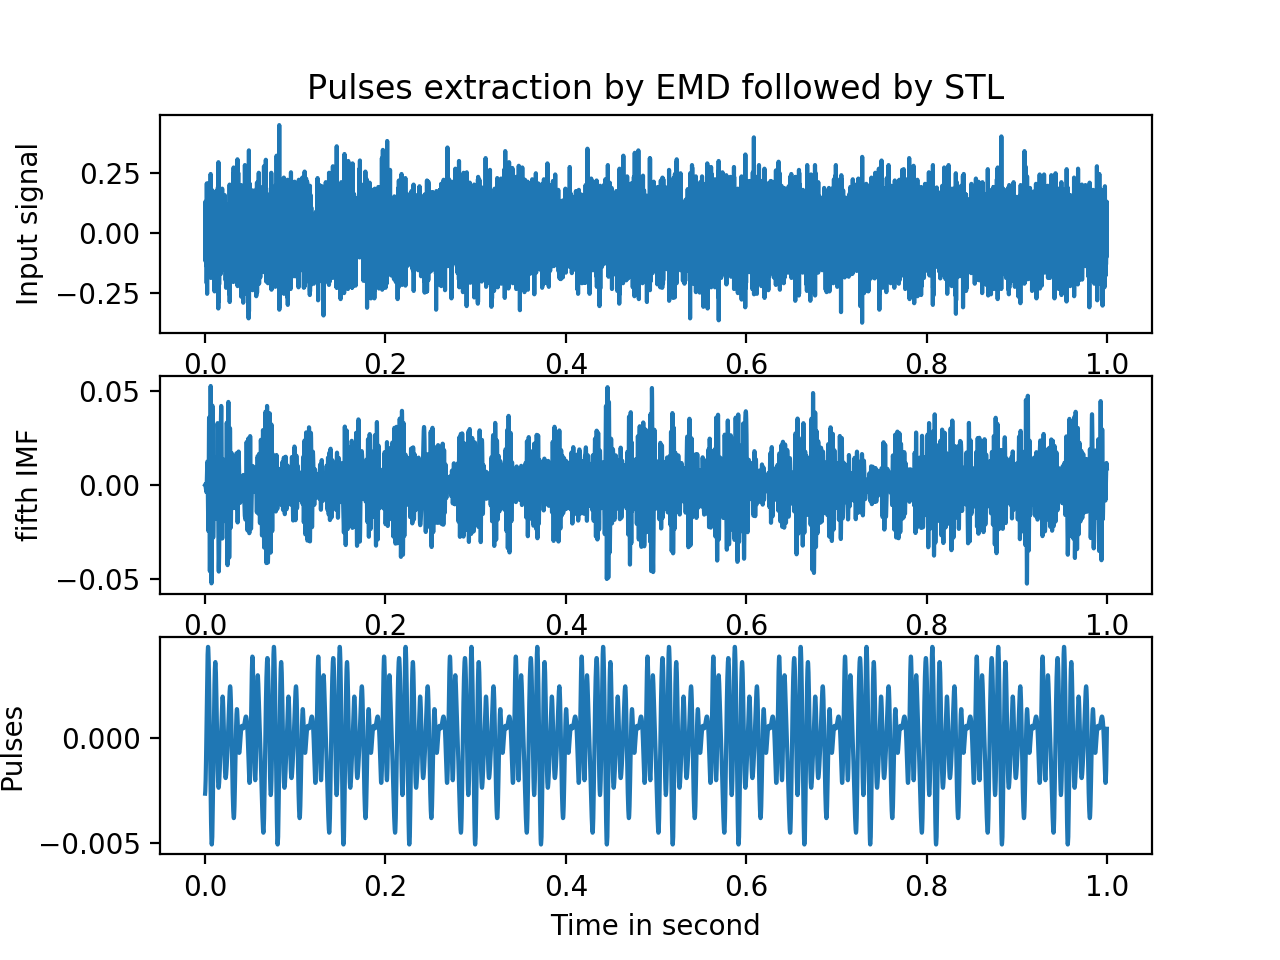
\includegraphics[width=0.6\linewidth]{emd-stl}
		%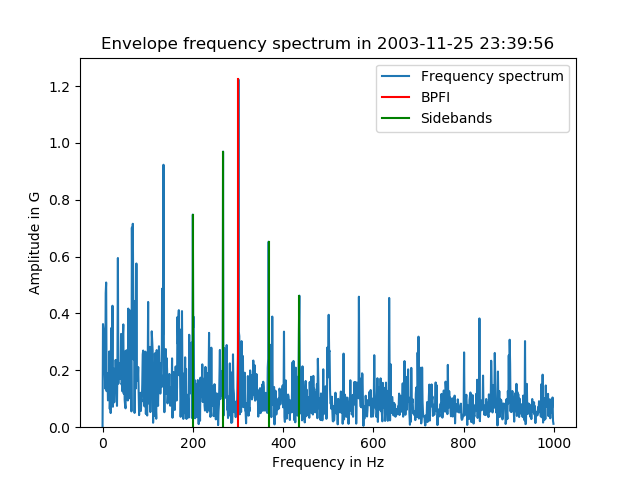
\includegraphics[width=0.45\linewidth]{bpfi_sidebands}
		%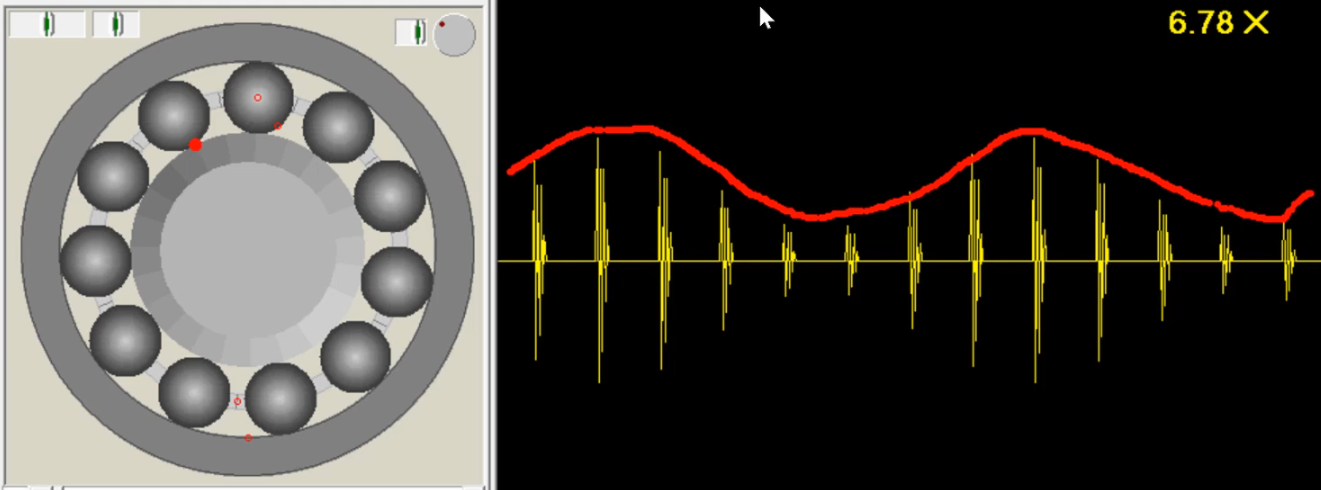
\includegraphics[width=0.8\linewidth]{inner-race2}
		%\caption{}
		%\label{fig:datascience}
	\end{figure}
\end{frame}

%%%%%%%%%%%%%%%%%%%%%%%%%%%%%%%%%%%%%%%%%%%%%%%%%%%%%%%%%



\begin{frame}
	\frametitle{Bearing faults are exposed through the power spectral density }
	\begin{equation}\label{eq:psd}
	PSD\left(s(t)\right) = E\left[ \frac{1}{N} \left\vert \sum_{t=1}^{N} s(t)e^{-i\omega t}\right\vert^{2}   \right]
	\end{equation}

	\begin{equation}
	\widehat{PSD}\left(s(t)\right) =  \frac{1}{N} \left\vert \sum_{t=1}^{N} s(t)e^{-i\omega t}\right\vert^{2}
	\end{equation}
	
\end{frame}

%%%%%%%%%%%%%%%%%%%%%%%%%%%%%%%%%%%%%%%%%%%%%%%%%%%%%%%%%

\begin{frame}
	\frametitle{A bearing inner race fault is exposed through the power spectral density }
	
	\begin{figure}[H]
		\centering
		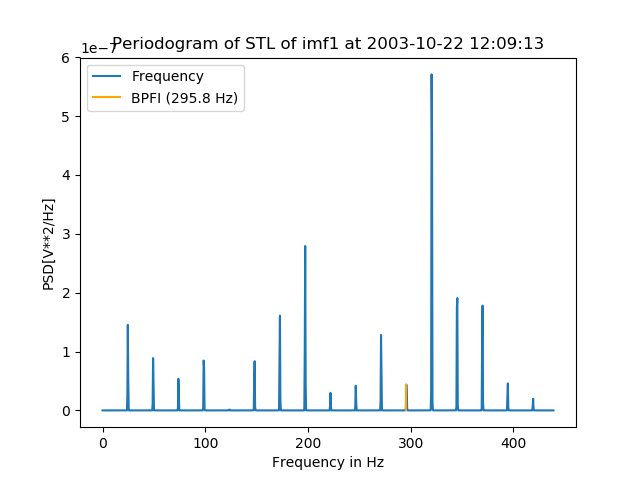
\includegraphics[width=0.45\linewidth]{start_imf1_bpfi}
		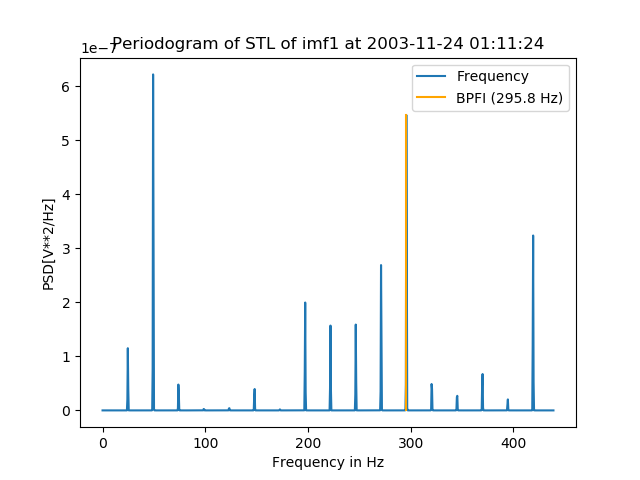
\includegraphics[width=0.45\linewidth]{end_imf1_bpfi}
		%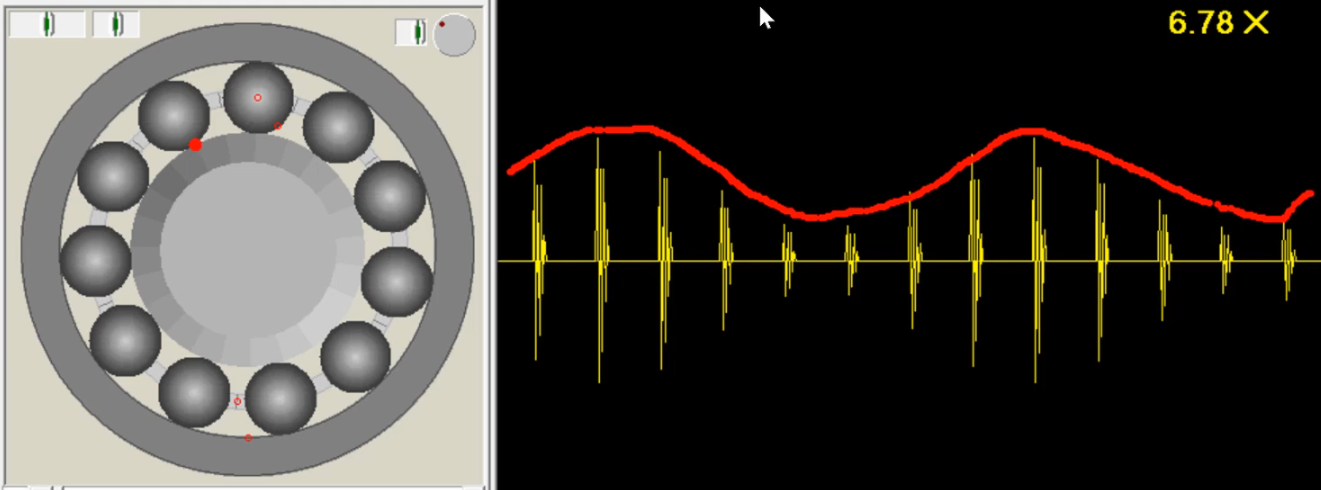
\includegraphics[width=0.8\linewidth]{inner-race2}
		%\caption{}
		%\label{fig:datascience}
	\end{figure}
\end{frame}

%%%%%%%%%%%%%%%%%%%%%%%%%%%%%%%%%%%%%%%%%%%%%%%%%%%%%%%%%




\begin{frame}
	\frametitle{A bearing outer race fault is exposed through the power spectral density }

	\begin{figure}[H]
		\centering
		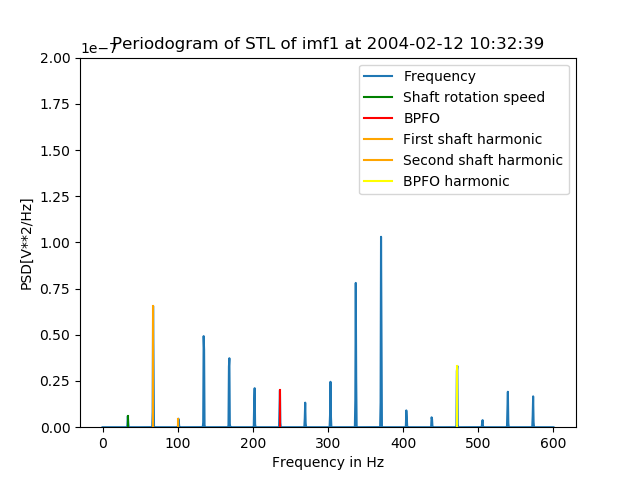
\includegraphics[width=0.45\linewidth]{start_imf1_bpfo}
		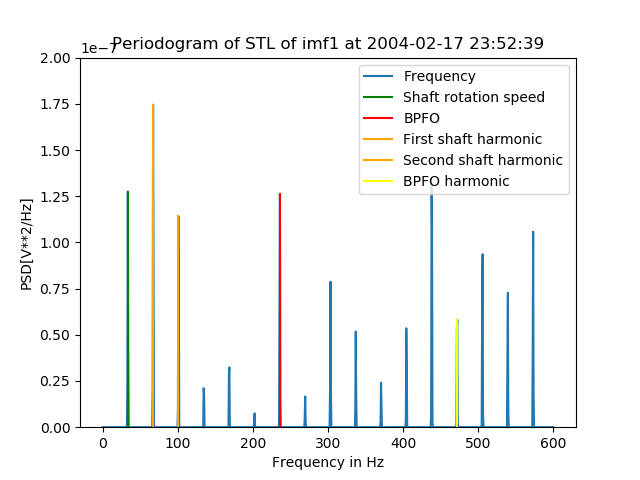
\includegraphics[width=0.45\linewidth]{end_imf1_bpfo}
	\end{figure}
\end{frame}

%%%%%%%%%%%%%%%%%%%%%%%%%%%%%%%%%%%%%%%%%%%%%%%%%%%%%%%%%


%%%%%%%%%%%%%%%%%%%%%%%%%%%%%%%%%%%%%%%%%%%%%%%%%%%%%%%%%


\begin{frame}
	\frametitle{The new method`s spectrum is noise free    }
	\begin{figure}[H]
		\centering
		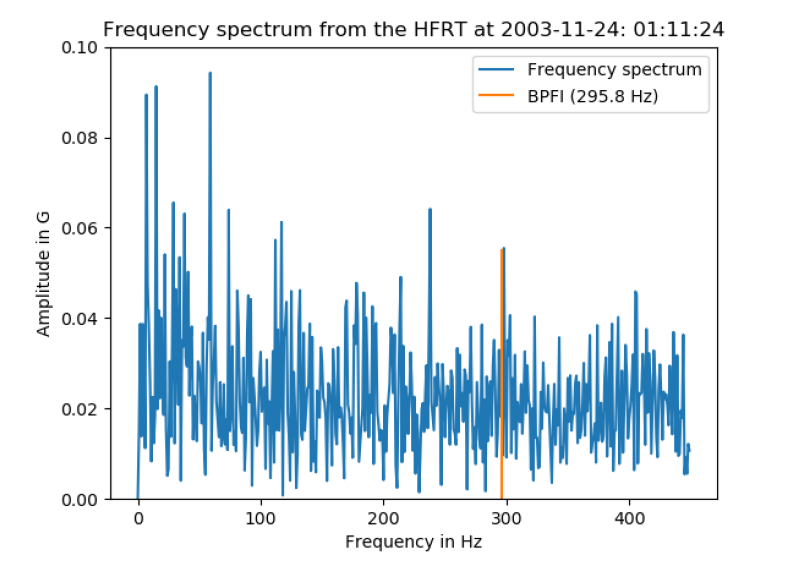
\includegraphics[width=0.5\linewidth]{method1}
		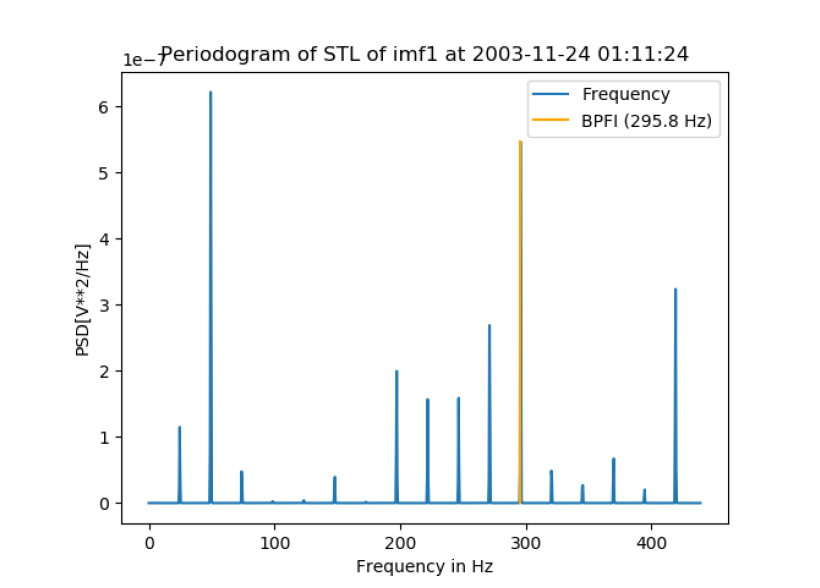
\includegraphics[width=0.5\linewidth]{method2}
		%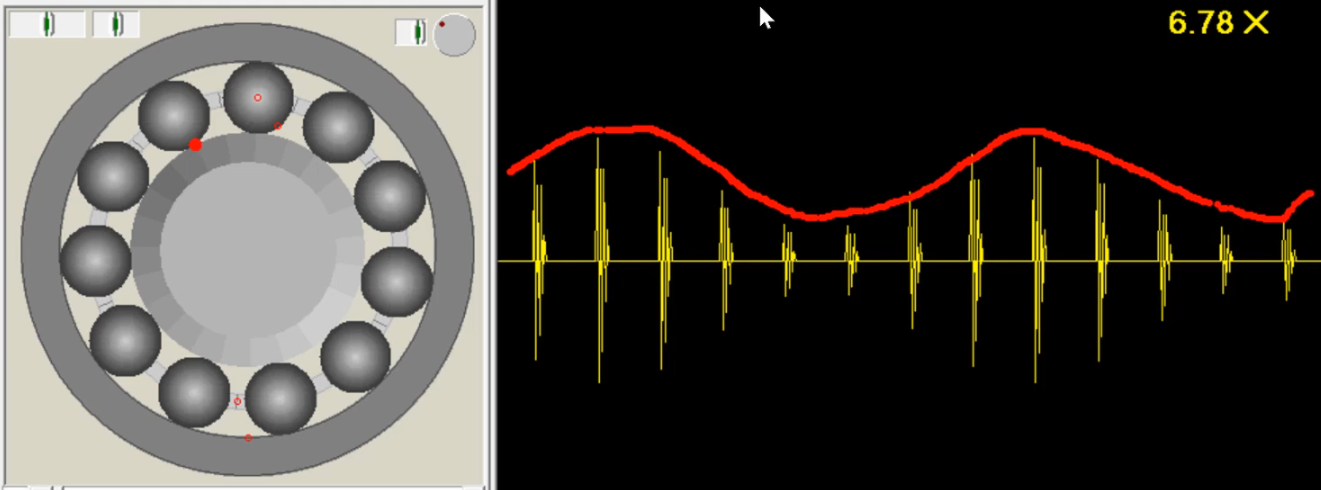
\includegraphics[width=0.8\linewidth]{inner-race2}
		%\caption{}
		%\label{fig:datascience}
	\end{figure}
\end{frame}

%%%%%%%%%%%%%%%%%%%%%%%%%%%%%%%%%%%%%%%%%%%%%%%%%%%%%%%%%


\begin{frame}
	\frametitle{Conclusion }
	\begin{itemize}
		\item The High Frequency resonance is still the state-of-the-art method 
		\item The proposed method adds value to bearing fault detection 
		\item Extend the thesis to other bearing faults
		\item Apply the method to bearings in industrial production
	\end{itemize}
\end{frame}

%%%%%%%%%%%%%%%%%%%%%%%%%%%%%%%%%%%%%%%%%%%%%%%%%%%%%%%%%


\end{document}

